\section{\method}
\label{sec:method}
% Framework overview (raster, 2026-10-25; replaces the B1-only TikZ overview kept in figs/fig_overview_b1_tikz.tex).
% 2026-10-27: material column relabelled (external appearance backend + planned constrained fusion) and a status note for G,
% by figs/src/relabel_framework.py from the user's original figs/src/fig_overview_framework_user.png.
% The caption states which boxes produce the results reported in this paper and which are under test, negative or planned.
\begin{figure*}[t]
\centering
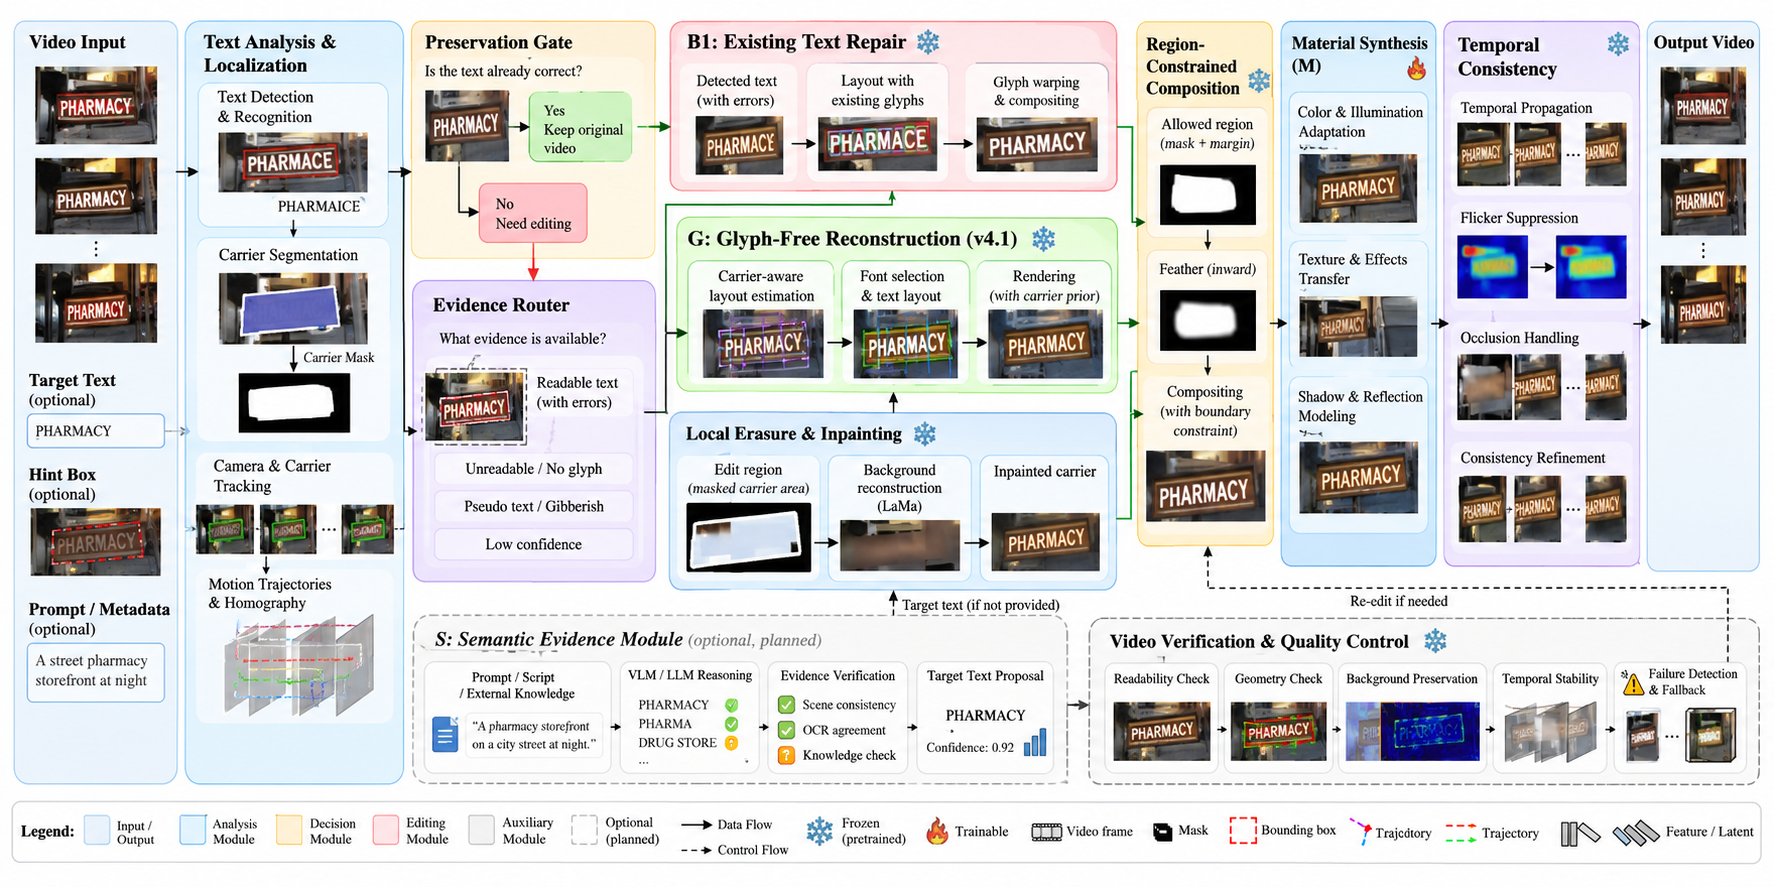
\includegraphics[width=\linewidth]{figs/fig_overview_framework.png}
\caption{\textbf{\method framework and the scope of this paper.} Text analysis reads and tracks the text and its carrier; the preservation gate returns the clip unchanged when the text already reads the target; otherwise the evidence available decides between repairing the existing text (B1) and glyph-free reconstruction (G); local erasure and a region-constrained compositor keep every edit inside the allowed region. \emph{Status:} all reported results come from the frozen B1 path; its only appearance step is the non-parametric source appearance transport, nothing is trained, and of the temporal box only carrier-anchored propagation belongs to it. G failed its sealed test and is exploratory (\cref{sec:exp_neg}). The appearance backend is an external model~\cite{zeng2026steervte} used only in Banksy-V (\cref{sec:exp_hybrid}); M, S, the router and the verification loop are planned, and a trained material generator was negative.}
\label{fig:overview}
\end{figure*}


\method takes a generated clip $V=\{I_t\}_{t=1}^{T}$, a target string $s$ and a hint box $b$ (\cref{sec:task}) and returns a clip $\hat V$ that differs from $V$ only inside the text region. \Cref{fig:overview} summarises the pipeline; all components are classical or pre-trained and nothing is trained for the task. We describe the steps in order and give thresholds and implementation details in the supplement.

\subsection{Reading the text and tracking its carrier}
\label{sec:read}
We run an off-the-shelf OCR system (EasyOCR~\cite{easyocr}, CRAFT detection~\cite{baek2019craft} and CRNN recognition~\cite{shi2017crnn}) on every frame and keep the boxes that overlap $b$. Boxes are grouped into text rows, and the frame whose rows best match $s$ (normalised edit similarity) becomes the reference frame $t^\star$. The text is printed on, or emitted by, a physical \emph{carrier}---a sign, a poster, a screen---so we track the carrier rather than the glyphs: SIFT keypoints~\cite{lowe2004sift} are matched between $I_{t^\star}$ and every $I_t$ inside a window one text-box size larger on each side of the reference quad, and a RANSAC~\cite{fischler1981ransac} homography $H_t$ is estimated (ratio test 0.75, reprojection threshold 2.5\,px, at least 10 inliers). When a frame fails, $H_t$ falls back to the quad-to-quad homography between the OCR boxes. Everything that is placed on the carrier later---erased background, glyphs, masks---is placed once in the reference frame and carried to frame $t$ by $H_t$, which removes per-frame jitter of the OCR boxes from the output.

\subsection{Preservation gate}
\label{sec:pres}
Generated text is often already correct, and any edit can only make such a clip worse. The preservation gate returns $\hat V=V$ when the OCR evidence across frames shows that the clip already reads $s$: the complete target is read in at least 85\% of the frames, wrong readings occur in at most 5\%, the reading lies inside the hint box, at most 10\% of the frames contain extra boxes, and the reading of all boxes inside the hint box, concatenated in reading order, equals $s$ in at least 90\% of the correct frames. The last condition prevents skipping when the target appears next to other, garbled text (\eg, a correct word above a garbled subtitle). The gate uses only the OCR of the pipeline, never the evaluation reader (\cref{sec:metrics}), and when the evidence is insufficient the clip is edited: the gate trades recall for safety. In the final run it skips \rSkipped{} of the 526 clips (9\%), all of which the independent reader confirms as correct.

\subsection{Localization gate and layout}
\label{sec:loc}
If the old glyphs can be localised reliably, the new text should inherit their size, colour and baseline. We estimate a glyph \emph{instance} in the reference frame: the ink mask (colour clustering inside the rows), the ink and ground colours, the letter height, the number of letters and the letter band. The localization gate accepts the instance only if it contains at least three letters (two for Chinese), the local contrast between ink and inter-letter ground exceeds 40 in CIELAB, the letter height is between 0.3 and 1.0 of the OCR box height, and the OCR rows did not require a fallback grouping. Otherwise the clip falls back to a \emph{box layout} that fills the tracked box with legible text. In the final run, \rBoxPolicy{} of the \rOursCollatN{} clips that \method edits (35\%) take the box layout.

With an accepted instance, the target is laid out on the letter band: the cap height equals the measured letter height, the string keeps its natural aspect ratio in the selected font, and it is centred on the old text; a target wider than the old line may extend the line by up to $1.35\times$ before its height is reduced. The band is oriented like the OCR quad, which for most detectors is axis-aligned---a limitation we return to in \cref{sec:limits}. Stacked text keeps its rows: the target is split into lines following the word counts of the detected rows, and each line is laid out on its own row instance.

\subsection{Erasure and deterministic rendering}
\label{sec:render}
\paragraph{Erasure.} The old glyphs are removed once, in the reference frame: the ink mask (closed, and extended by the bright pixels of glowing text) is dilated by $\min(0.3h,\max(10,0.18h))$ pixels for text height $h$, flat grounds are pre-filled with their median colour, and the hole is inpainted with LaMa~\cite{suvorov2022lama}. The erased background is then carried to every frame by $H_t$, with a per-frame, per-channel gain fitted on a ring around the hole and smoothed over five frames, so that exposure changes follow without per-frame inpainting flicker.

\paragraph{Font matching.} The new glyphs are rendered, not generated. The font is chosen from a library of 33 Latin and 8 Chinese families (variable fonts expanded over their weights) by comparing stroke statistics of the warped old ink mask with those of each candidate rendered in the same layout; script and display faces are admitted only when they are clearly better (distance below 0.6 of the best plain face). Because the target string is drawn by a font rasteriser, its spelling is exact by construction.

\paragraph{Photometry.} The glyph colour follows the per-frame ink colour of the old text (running median over seven frames) modulated by a low-frequency shading field estimated from the old strokes in canonical text coordinates, and glowing text receives a soft halo. The canvas is warped to every frame with $H_t$ and composited over the erased background.

\subsection{Appearance gate and source appearance transport}
\label{sec:sat}
Rendering gives the right letters, but on emissive carriers---neon, lightboxes, screens---the old glyphs carry glow, bloom and inner structure that a flat fill cannot reproduce. SAT transports this appearance from the old glyphs to the new ones without regenerating the region. Let $B$ be the erased background, $I$ the reference frame and $d(x)$ the signed distance of pixel $x$ to the boundary of the old glyphs, in units of the letter height. On the old text we fit, per distance bin $k$ and per channel, a multiplicative-plus-additive light-transport operator
\begin{equation}
I(x)\approx m_k\,B(x)+a_k,\qquad k=k(d(x)),
\label{eq:sat}
\end{equation}
over the support $d\le0.6$, and apply it to the new glyphs with their own distance field, $\hat I(x)=m_{k(\hat d(x))}B(x)+a_{k(\hat d(x))}$. On the old text, this family reconstructs the source better than an additive-only operator, a distance-indexed replacement or a flat fill (cross-validated CIELAB error 17.2 vs.\ 25.9, 27.6 and 29.7; best on 45 of 52 clips; supplement), which is why we keep both terms.

SAT is applied only behind an \emph{appearance gate} with two conditions: the text must be emissive (ink brighter than its ground, or a detected glow on the carrier), and the operator must generalise across the text---fitted on one half and tested on the other, in both directions, its error must stay below 0.75 of the flat-fill error. In the final run, SAT is enabled on \rSatOn{} clips (10\%); it is never applied to box-layout clips, whose instance evidence is weak by definition.

\subsection{Compositing}
The output differs from the input only where the erasure mask or the new glyphs (with halo) are non-zero; elsewhere the input pixels are copied, so the only residual outside the text region is the re-encoding of the video.
